% Report: how the reset rule is chosen (offline screening at fixed collapse rates), what the screen found, and the live runs of the finalists.
% Needs booktabs, amsmath, graphicx, enumitem, url. Table numbers come from out/results/screen_resets_stress/*SHT*.json (screen) and out/results/reset_live/*/report/*.json (live runs);
% the figures are copied from out/results/reset_live/*/report/ into figures/reset_live/.
\documentclass[10pt]{article}
\usepackage[margin=2.3cm]{geometry}
\usepackage{booktabs}
\usepackage{amsmath}
\usepackage{graphicx}
\usepackage{enumitem}
\usepackage[hyphens]{url}
\urlstyle{tt}
\setlist{nosep,leftmargin=1.4em}
\newcommand{\rl}[1]{\texttt{#1}}
\newcommand{\vit}{ViT-B/16}
\newcommand{\rn}{ResNet-50}

\title{Choosing a reset rule: offline screening and live runs at fixed collapse rates}
\author{Dynamic Duos, \vit{} + \rn{} V1, Tent, Vanilla DD}
\date{26 October 2026}

\begin{document}
\maketitle

\section{Question and setting}
A reset puts a member back to its source weights. We want a rule that flags a collapsing member soon and rarely resets a healthy one, using only the label-free signal the gate already computes.
We compare 15 detector families on stored runs (the \emph{screen}), then run the five best live with real resets (Section~\ref{sec:live}).

The setting is the one of the gate-stress experiments: Vanilla DD (each member adapts with Tent on its own entropy, the gate sits outside the loop), the nuclear-norm proxy with proxy batch $b_t = 256$, gate $\beta = 2$ ($\beta$ changes neither the members nor the proxy values).
The learning rates are \emph{fixed} to values that collapse both members (stress pair: \vit{} $1.4{\cdot}10^{-4}$, \rn{} $5{\cdot}10^{-4}$). The rates tuned for stability without resets (the 04b rates) are too low for a resetting scheme, so rates are not tuned here.

\section{The rules}
\paragraph{Signals.} Each proxy batch gives each member a proxy value $r^{(m)}_t \in (0,1)$; let $s^{(m)}_t = \operatorname{logit}(r^{(m)}_t)$ (clipped). A member's rule watches either its own score (\emph{own}, $s^{(m)}_t$), its gap to the partner (\emph{gap}, $s^{(m)}_t - s^{(m')}_t$, antisymmetric between the two members), or either of the two (\emph{both}: gap OR own, same parameters).

\paragraph{Procedures.} Five one-sided detectors, each standardized: the deviation is divided by a running standard deviation of the signal (exponential rate $0.01$, taken before the new value enters), so thresholds are in noise units. For the first $W_0$ batches after (re)start a detector only learns its reference mean $m_0$. With $\sigma$ the running standard deviation, a detector alarms when
\begin{itemize}
  \item \textbf{level}: $(x_t - m_0)/\sigma < \tau$;
  \item \textbf{imm\_vs\_ema}: $\bar x_{t-1} - x_t > \delta\sigma$, with $\bar x$ an exponential average (rate $\alpha$) started at $m_0$;
  \item \textbf{fast\_vs\_slow}: $\bar x^{\text{slow}}_t - \bar x^{\text{fast}}_t > \delta\sigma$, two exponential averages started at $m_0$;
  \item \textbf{slope}: the least-squares slope over the last $W$ values, divided by $\sigma$, is below $-\gamma$ for $k$ consecutive batches;
  \item \textbf{cusum}: $S_t = \max(0, S_{t-1} + (\mu - x_t)/\sigma - \nu) > h$, with $\mu$ the frozen warm-up mean (own) or $0$ (gap).
\end{itemize}
\paragraph{Controller.} A member is flagged when any detector of its rule alarms. A flagged member has its detectors restarted (and the partner's gap detector, since that is built from the flagged member's proxy), and cannot be flagged again for $K = W_0$ batches.

\paragraph{Grid.} Table~\ref{tab:grid} lists the settings. Three signal choices $\times$ five procedures give 15 families; that makes 232 settings per signal choice (16 + 48 + 48 + 72 + 48) and \textbf{696} in total.

\begin{table}[ht]
  \centering\small
  \caption{Grid of one family; every row is crossed with $W_0 \in \{20, 50\}$.}
  \label{tab:grid}
  \begin{tabular}{@{}l p{6.2cm} l l@{}}
    \toprule
    procedure & swept parameters & threshold & values \\
    \midrule
    level        & ---                                            & $\tau$   & $-1, -1.5, -2, -3, -4, -5, -6, -8$ \\
    imm\_vs\_ema & $\alpha \in \{0.01, 0.05, 0.1\}$               & $\delta$ & $1, 1.5, 2, 3, 4, 5, 6, 8$ \\
    fast\_vs\_slow & $(\alpha_f, \alpha_s) \in \{(.05,.005), (.1,.01), (.2,.02)\}$ & $\delta$ & $1, 1.5, 2, 3, 4, 5, 6, 8$ \\
    slope        & $W \in \{16, 32, 64\}$, $k \in \{1, 4\}$       & $\gamma$ & $.005, .01, .02, .05, .1, .2$ \\
    cusum        & $\nu \in \{0.25, 0.5, 1\}$                     & $h$      & $2, 4, 8, 12, 16, 24, 32, 48$ \\
    \bottomrule
  \end{tabular}
\end{table}

\section{Data}
Every run is Vanilla DD without any reset, stored together with a frozen-member run on the same images and the gate's per-batch proxy values. A rule is \emph{replayed} on these proxy sequences exactly as the live controller would run, but the trajectory is not changed (the reset model cannot be simulated offline), so only each member's \emph{first} collapse is measured. The live runs rank the finalists.

\begin{table}[ht]
  \centering\small
  \caption{The three sets of runs. S: held-out stream (speckle, Gaussian blur, spatter, saturate; severity 5, 50k images each; 4 rounds, round $r$ rotated by $r$), 4 rotations $\times$ 2 seeds. H: the same stream at full length, rotations 0 and 2, seed 0. T: the test stream, seeds 0--2. A member-batch is one proxy batch of one member (a stream contributes two); ``healthy'' = outside every degraded stretch (see below).}
  \label{tab:data}
  \begin{tabular}{@{}l l l r r r r@{}}
    \toprule
    set & ViT rate & ResNet rate & streams & member-batches & healthy & events \\
    \midrule
    S (calibration) & $1.4{\cdot}10^{-4}$  & $5{\cdot}10^{-4}$   & 8 & 19,328 & 34\% & 23 \\
    H (calibration) & $1.26{\cdot}10^{-5}$ & $2.2{\cdot}10^{-5}$ & 2 & 12,500 & 99\% & 3 \\
    T (test)        & $1.4{\cdot}10^{-4}$  & $5{\cdot}10^{-4}$   & 3 & 10,948 & 54\% & 9 \\
    \bottomrule
  \end{tabular}
\end{table}
\noindent S stops 20,000 images after both members are dead, so most of each S run is degraded: it supplies 23 of the 26 calibration events but only a third of the healthy time. H is the stable pair: it supplies the healthy time, and almost every alarm in it is false (its only events are 3 short dips of the \rn{}). T is never used for a choice.

\section{Labels and metrics}\label{sec:labels}
Labels are used only for evaluation; they never reach a rule.
\begin{itemize}
  \item A member is \emph{degraded} at batch $t$ if it is clearly worse than its own frozen (non-adapting) copy on the same images. Three label parameters define ``clearly'':
  \begin{itemize}
    \item $M$, the \emph{smoothing window} (in batches): the accuracy difference ``adapted minus frozen'' is averaged over $M$ batches. Default $M = 8$.
    \item $\delta$, the \emph{margin} (in accuracy points; 1 pt = one percentage point): the member is degraded when that smoothed difference is below $-\delta$. Default $\delta = 1$ pt.
    \item $L$, the \emph{minimum stretch length} (in batches): a run of consecutive degraded batches counts only if it lasts at least $L$ batches. Such a stretch is a \emph{collapse event} and its first batch is the \emph{onset}; shorter dips are ignored. Default $L = 16$.
  \end{itemize}
  \item \textbf{Delay}: batches from the onset to the first alarm in the stretch (an alarm up to 8 batches before the onset counts as delay $0$). A stretch with no alarm is a \textbf{miss} and is charged its whole length as delay.
  \item \textbf{False alarm}: an alarm outside every stretch (less the 8-batch slack). The \textbf{false-alarm rate} is false alarms per 1,000 member-batches, all batches counted (degraded ones too).
\end{itemize}
One batch is 256 images, so a delay of 100 batches is 25.6k images. A \textbf{false-alarm budget} of $1$ per 1,000 allows one unneeded reset per member per 256k images (about 3 per member on an 800k-image stream).
Without a budget the comparison is meaningless: a rule that fires every batch has zero delay. A budget fixes the cost of a reset on a healthy member and lets each family compete at its best setting.

\section{Selection protocol}
\begin{enumerate}
  \item Replay all 696 settings on the \textbf{calibration pool}: S and H together (10 streams, 31,828 member-batches, 26 events: 8 \vit{}, 18 \rn{}). Events, misses, delays, false alarms and batches are summed over all (stream, member) pairs.
  \item For each family and each budget $b \in \{0.5, 1, 2\}$ keep the settings whose pooled false-alarm rate is at most $b$, and take the one with the lowest mean delay (ties: fewer misses, then fewer false alarms). One setting, one threshold, for both members.
  \item \textbf{Freeze} that setting and score it once on the \textbf{test streams} T. Nothing is chosen on T and the budget is not enforced there: a test false-alarm rate above the budget measures how well the setting transfers.
  \item Report the budget-1 table, the other budgets, per-member scores, and the sensitivity of the ranking to the labels ($M \in \{4, 8, 16\}$ batches, $\delta \in \{0.5, 1, 2\}$ pt, $L \in \{8, 16, 32\}$ batches; one parameter changed at a time).
\end{enumerate}

\section{Screening results}
\paragraph{Budget 1 (Table~\ref{tab:b1}).} The three leaders on the calibration pool are \rl{gap\_fast\_vs\_slow}, \rl{own\_fast\_vs\_slow} and \rl{own\_cusum}. On the test streams \rl{own\_fast\_vs\_slow} is best: delay 23 batches (about 6k images), 2 of 9 events missed, 0.27 false alarms per 1,000.
\rl{gap\_fast\_vs\_slow} has a similar delay but 1.19 false alarms on the test streams, above the budget. \rl{both\_cusum} and \rl{gap\_cusum} have no setting within any budget: their lowest false-alarm rate on the grid is $3.8$ per 1,000, so their threshold grid is too low to conclude anything about the rule.

\begin{table}[ht]
  \centering\small
  \caption{Budget of 1 false alarm per 1,000 member-batches: the setting chosen on the calibration pool (S+H), scored there and, frozen, on the test streams T. Delay in 256-image batches (a miss is charged its whole length), miss = missed events / events, FA = false alarms per 1,000 member-batches. Sorted by calibration delay.}
  \label{tab:b1}
  \begin{tabular}{lrrrrrr}
    \toprule
    & \multicolumn{3}{c}{calibration (26 events)} & \multicolumn{3}{c}{test (9 events)} \\
    \cmidrule(lr){2-4} \cmidrule(lr){5-7}
    rule & delay & miss & FA & delay & miss & FA \\
    \midrule
    \rl{gap\_fast\_vs\_slow} & 110 & 0.35 & 0.91 & 32 & 0.33 & 1.19 \\
    \rl{own\_fast\_vs\_slow} & 113 & 0.31 & 0.69 & 23 & 0.22 & 0.27 \\
    \rl{own\_cusum} & 133 & 0.31 & 0.72 & 59 & 0.33 & 0.00 \\
    \rl{own\_level} & 147 & 0.31 & 0.69 & 96 & 0.33 & 0.00 \\
    \rl{both\_fast\_vs\_slow} & 153 & 0.38 & 0.72 & 450 & 0.67 & 0.00 \\
    \rl{gap\_slope} & 156 & 0.38 & 0.31 & 553 & 1.00 & 0.09 \\
    \rl{both\_level} & 170 & 0.42 & 0.82 & 120 & 0.56 & 0.18 \\
    \rl{gap\_level} & 171 & 0.50 & 0.53 & 55 & 0.33 & 0.00 \\
    \rl{own\_imm\_vs\_ema} & 203 & 0.54 & 0.97 & 448 & 0.56 & 0.64 \\
    \rl{both\_slope} & 214 & 0.58 & 0.75 & 401 & 0.78 & 0.27 \\
    \rl{own\_slope} & 215 & 0.62 & 0.75 & 529 & 0.89 & 0.27 \\
    \rl{both\_imm\_vs\_ema} & 215 & 0.54 & 0.94 & 553 & 1.00 & 0.27 \\
    \rl{gap\_imm\_vs\_ema} & 319 & 0.73 & 0.72 & 553 & 1.00 & 0.09 \\
    \rl{both\_cusum} & \multicolumn{6}{c}{no setting within the budget} \\
    \rl{gap\_cusum} & \multicolumn{6}{c}{no setting within the budget} \\
    \bottomrule
  \end{tabular}
\end{table}

\paragraph{Selected settings of the leaders (Table~\ref{tab:sel}).} The own and gap \rl{fast\_vs\_slow} leaders use the slowest pair of averages of the grid and the lowest threshold; \rl{both\_fast\_vs\_slow} uses a faster pair and $\delta = 1.5$.

\begin{table}[ht]
  \centering\small
  \caption{Frozen settings of the five leaders at budget 1 and their calibration false-alarm rate.}
  \label{tab:sel}
  \begin{tabular}{lrllr}
    \toprule
    rule & $W_0$ & parameters & threshold & FA (calib.) \\
    \midrule
    \rl{gap\_fast\_vs\_slow} & 50 & $(\alpha_f,\alpha_s)$=(0.05, 0.005) & $\delta = 1$ & 0.91 \\
    \rl{own\_fast\_vs\_slow} & 20 & $(\alpha_f,\alpha_s)$=(0.05, 0.005) & $\delta = 1$ & 0.69 \\
    \rl{own\_cusum} & 50 & $\nu$=0.25 & $h = 2$ & 0.72 \\
    \rl{own\_level} & 50 & --- & $\tau = -1.5$ & 0.69 \\
    \rl{both\_fast\_vs\_slow} & 20 & $(\alpha_f,\alpha_s)$=(0.1, 0.01) & $\delta = 1.5$ & 0.72 \\
    \bottomrule
  \end{tabular}
\end{table}

\paragraph{Across budgets (Table~\ref{tab:bud}).} \rl{fast\_vs\_slow} is the one procedure in the top five of the calibration pool at all three budgets (any signal choice). \rl{imm\_vs\_ema} is the weakest family: it compares a sample with its own moving average, so a slow ramp drags the average along and is not seen (the \rn{} decays gradually). \rl{slope} is the best at budget 2 on the calibration pool but is erratic on the test streams (own\_slope and gap\_slope at budget 1 miss most or all test events).
The ranking changes with the budget: \rl{gap\_fast\_vs\_slow} leads at 0.5 and 1, \rl{own\_slope} at 2 (it is 11th at budget 1). Settings that are best on the calibration pool can also miss on T: \rl{both\_fast\_vs\_slow} has delay 450 on T at budget 1 (its \rn{} events are missed) but 28 at budget 0.5.

\begin{table}[ht]
  \centering\small
  \caption{Mean delay (256-image batches, misses charged their whole length) of each family's chosen setting at the three budgets, on the calibration pool and, frozen, on the test streams. Best per calibration column in bold; -- = no setting within the budget.}
  \label{tab:bud}
  \begin{tabular}{lrrrrrr}
    \toprule
    & \multicolumn{3}{c}{calibration} & \multicolumn{3}{c}{test} \\
    \cmidrule(lr){2-4} \cmidrule(lr){5-7}
    budget (FA per 1,000) & 0.5 & 1 & 2 & 0.5 & 1 & 2 \\
    \midrule
    \rl{own\_level} & 164 & 147 & 141 & 161 & 96 & 67 \\
    \rl{gap\_level} & 232 & 171 & 119 & 85 & 55 & 31 \\
    \rl{both\_level} & 296 & 170 & 143 & 220 & 120 & 24 \\
    \addlinespace
    \rl{own\_imm\_vs\_ema} & 488 & 203 & 109 & 553 & 448 & 243 \\
    \rl{gap\_imm\_vs\_ema} & 339 & 319 & 216 & 553 & 553 & 441 \\
    \rl{both\_imm\_vs\_ema} & 488 & 215 & 215 & 553 & 553 & 553 \\
    \addlinespace
    \rl{own\_fast\_vs\_slow} & 230 & 113 & 102 & 49 & 23 & 14 \\
    \rl{gap\_fast\_vs\_slow} & \textbf{147} & \textbf{110} & 85 & 450 & 32 & 13 \\
    \rl{both\_fast\_vs\_slow} & 154 & 153 & 74 & 28 & 450 & 19 \\
    \addlinespace
    \rl{own\_slope} & 488 & 215 & \textbf{54} & 553 & 529 & 30 \\
    \rl{gap\_slope} & 156 & 156 & 80 & 553 & 553 & 130 \\
    \rl{both\_slope} & 488 & 214 & 116 & 553 & 401 & 457 \\
    \addlinespace
    \rl{own\_cusum} & 149 & 133 & 133 & 121 & 59 & 59 \\
    \rl{gap\_cusum} & -- & -- & -- & -- & -- & -- \\
    \rl{both\_cusum} & -- & -- & -- & -- & -- & -- \\
    \bottomrule
  \end{tabular}
\end{table}

\paragraph{Per member (Table~\ref{tab:mem}).} The two \rl{fast\_vs\_slow} leaders catch the \vit{} within 11--32 batches (3k--8k images) on both calibration and test, and miss none of its long collapses; \rl{own\_cusum} and \rl{own\_level} take 21--85. The \rn{} decays gradually, so its onset (1 point below frozen) comes long before any detector can tell: calibration delays are around 150 batches, including the charge for missed dips.
Missed events are almost all short: for \rl{own\_fast\_vs\_slow} the 8 calibration misses are \rn{} stretches of 16, 17, 26, 31, 43, 58, 97 and 265 batches, and the 2 test misses are \vit{} dips of 35 and 38 batches; every stretch of 300 batches or more is detected. Whether a short dip that recovers on its own should trigger a reset is a modelling choice (see below).

\begin{table}[ht]
  \centering\small
  \caption{Per member at budget 1: mean delay in batches (missed / events). Calibration: 8 \vit{} and 18 \rn{} events; test: 5 and 4.}
  \label{tab:mem}
  \begin{tabular}{lrrrr}
    \toprule
    & \multicolumn{2}{c}{calibration} & \multicolumn{2}{c}{test} \\
    \cmidrule(lr){2-3} \cmidrule(lr){4-5}
    rule & \vit{} & \rn{} & \vit{} & \rn{} \\
    \midrule
    \rl{gap\_fast\_vs\_slow} & 11 (0/8) & 154 (9/18) & 26 (2/5) & 39 (1/4) \\
    \rl{own\_fast\_vs\_slow} & 32 (0/8) & 149 (8/18) & 28 (2/5) & 18 (0/4) \\
    \rl{own\_cusum} & 21 (0/8) & 183 (8/18) & 62 (2/5) & 56 (1/4) \\
    \rl{own\_level} & 22 (0/8) & 203 (8/18) & 85 (2/5) & 111 (1/4) \\
    \rl{both\_fast\_vs\_slow} & 16 (0/8) & 213 (10/18) & 27 (2/5) & 978 (4/4) \\
    \bottomrule
  \end{tabular}
\end{table}

\paragraph{Label sensitivity (Table~\ref{tab:sens}).} Under $M$ and the margin $\delta$ the delays move by at most 12\%; \rl{own\_cusum} stays behind the two \rl{fast\_vs\_slow} rules in every variant, and those two stay within 12 batches of each other. The minimum stretch length $L$ moves the miss rate most, because it decides how many short dips are counted as events.

\begin{table}[ht]
  \centering\small
  \caption{The three leaders' frozen settings re-scored on the calibration pool under other degradation labels. Each row changes one label parameter of Section~\ref{sec:labels} from the base row: $M$ = smoothing window (batches), $\delta$ = margin (accuracy points below the frozen member), $L$ = minimum stretch length (batches). Cell = mean delay in 256-image batches / miss rate (missed events / events).}
  \label{tab:sens}
  \begin{tabular}{lrrr}
    \toprule
    labels & \rl{gap\_fast\_vs\_slow} & \rl{own\_fast\_vs\_slow} & \rl{own\_cusum} \\
    \midrule
    base ($M{=}8$, $\delta{=}1$ pt, $L{=}16$) & 110 / 0.35 & 113 / 0.31 & 133 / 0.31 \\
    $M = 4$ & 98 / 0.39 & 109 / 0.39 & 127 / 0.36 \\
    $M = 16$ & 115 / 0.35 & 118 / 0.31 & 139 / 0.31 \\
    $\delta = 0.5$ pt & 99 / 0.45 & 101 / 0.42 & 118 / 0.42 \\
    $\delta = 2$ pt & 100 / 0.37 & 99 / 0.33 & 119 / 0.33 \\
    $L = 8$ & 78 / 0.55 & 80 / 0.53 & 94 / 0.53 \\
    $L = 32$ & 125 / 0.23 & 129 / 0.18 & 153 / 0.18 \\
    \bottomrule
  \end{tabular}
\end{table}

\section{Live runs with resets}\label{sec:live}
The screen replays rules on stored runs, so it cannot show what a reset does to the rest of the stream. We therefore ran the five leaders of Table~\ref{tab:sel} live: their frozen settings drive a controller that, when it flags a member, restores that member's source weights and clears its optimizer before the next batch (the gate keeps its buffer and is not reset).

\paragraph{Setup.} Vanilla DD with Tent, \vit{} at $1.4{\cdot}10^{-4}$ and \rn{} at $5{\cdot}10^{-4}$ (the stress pair: without resets both collapse), $\beta = 2$, whole streams, no early stop. Streams: the held-out stream (4 shifts $\times$ 4 rounds; opening shift 0 and 2; one seed) and the test stream (15 corruptions, standard order; seeds 0--2, which change the data order only). Conditions:
\begin{itemize}
  \item \textbf{No reset}, and the \textbf{frozen} duo (no adaptation) as the reference.
  \item The five \textbf{rules}, label-free.
  \item \textbf{Fixed schedule}: both members every $N$ adaptation steps (batch size 64): $N = 250, 500, 1000, 2000$ on held-out, $500$ and $1000$ on test ($1000$ is RDumb's period; $500$ was the best on held-out, by $0.1$ point). Label-free and blind.
  \item \textbf{Episodic}: both members and the gate restart at every shift boundary, the episodic protocol run as one stream. It is told where the shifts are, which no rule is: a reference.
  \item \textbf{Oracle}: uses the labels and a frozen copy of the pair stepped in lockstep; a member is reset once its accuracy over the last 8 proxy batches has stayed more than 1 point below its frozen copy's for 16 proxy batches in a row (the label definition of Section~\ref{sec:labels}, read causally). It cannot act before it has seen 16 degraded batches, so it is a reference, not a bound.
\end{itemize}
Each reset is audited afterwards: it is \emph{false} if the member was not more than 1 point below its frozen copy over the 8 proxy batches before it. A false reset costs adaptation progress but, as Table~\ref{tab:live} shows, is not necessarily harmful.
The loop was checked against the earlier loops: on the real models a live run without resets equals the earlier stress run over its first 12,800 images in every sample, the frozen copies equal a standalone frozen run, and a member's first batch after a reset equals the frozen member's.

\paragraph{Whole-stream accuracy (Table~\ref{tab:live}, Figures~\ref{fig:overlay-test} and~\ref{fig:overlay-held}).} Without a reset the duo collapses: 13.1\% on held-out and 24.2\% on test, against 52.1\% and 46.1\% for the frozen duo (on test seed 0 the \vit{} is below 5\% accuracy for 42\% of the stream and the \rn{} for 79\%). Every rule rescues it, ending 3.3 to 4.4 points above the frozen duo on held-out and 4.8 to 7.7 on test.

\begin{table}[t]
  \centering\footnotesize\setlength{\tabcolsep}{4pt}
  \caption{Live runs, Vanilla DD with Tent, \vit{} at $1.4{\cdot}10^{-4}$ and \rn{} at $5{\cdot}10^{-4}$, whole streams. Duo = mean accuracy (\%) of Vanilla DD over the whole stream (mean over 2 held-out runs, 3 test seeds; the spread over runs is at most 0.5 points and reflects the data order only); $\Delta$ = gain over the frozen duo on the same images; resets per 1,000 proxy batches as \vit{} / \rn{}; false = share of resets (\%) of a member that was not below its frozen copy. -- = not run. Rules in the order of Table~\ref{tab:b1}.}
  \label{tab:live}
  \begin{tabular}{@{}l rrrr rrrr@{}}
    \toprule
    & \multicolumn{4}{c}{held-out (2 runs)} & \multicolumn{4}{c}{test (3 seeds)} \\
    \cmidrule(lr){2-5} \cmidrule(lr){6-9}
    condition & duo & $\Delta$ & resets & false & duo & $\Delta$ & resets & false \\
    \midrule
    Frozen duo & 52.1 & -- & -- & -- & 46.1 & -- & -- & -- \\
    \midrule
    No reset & 13.1 & -38.9 & 0.0 / 0.0 & -- & 24.2 & -21.9 & 0.0 / 0.0 & -- \\
    \midrule
    \rl{gap\_fast\_vs\_slow} & 56.5 & +4.4 & 2.9 / 2.7 & 66 & 53.8 & +7.7 & 2.0 / 3.0 & 91 \\
    \rl{own\_fast\_vs\_slow} & 55.6 & +3.5 & 2.1 / 1.4 & 32 & 52.4 & +6.3 & 1.0 / 1.4 & 29 \\
    \rl{own\_cusum} & 55.7 & +3.6 & 3.0 / 1.3 & 44 & 51.8 & +5.7 & 0.7 / 1.5 & 5 \\
    \rl{own\_level} & 55.4 & +3.3 & 2.7 / 1.3 & 36 & 51.8 & +5.7 & 0.3 / 1.0 & 0 \\
    \rl{both\_fast\_vs\_slow} & 55.9 & +3.8 & 2.2 / 2.2 & 36 & 50.9 & +4.8 & 0.8 / 1.5 & 55 \\
    \midrule
    Every 250 steps & 54.3 & +2.2 & 16.0 / 16.0 & 100 & -- & -- & -- & -- \\
    Every 500 steps & 55.4 & +3.3 & 8.0 / 8.0 & 92 & 51.7 & +5.6 & 7.8 / 7.8 & 99 \\
    Every 1,000 steps & 55.3 & +3.2 & 3.8 / 3.8 & 73 & 52.7 & +6.6 & 3.8 / 3.8 & 95 \\
    Every 2,000 steps & 53.5 & +1.4 & 1.9 / 1.9 & 42 & -- & -- & -- & -- \\
    \midrule
    Episodic (every shift) & 56.4 & +4.3 & 4.8 / 4.8 & 88 & 53.3 & +7.2 & 4.8 / 4.8 & 90 \\
    Oracle (labels) & 56.9 & +4.8 & 2.1 / 2.2 & 0 & 52.6 & +6.4 & 2.3 / 1.7 & 0 \\
    \bottomrule
  \end{tabular}
\end{table}

\begin{figure}[t]
  \centering
  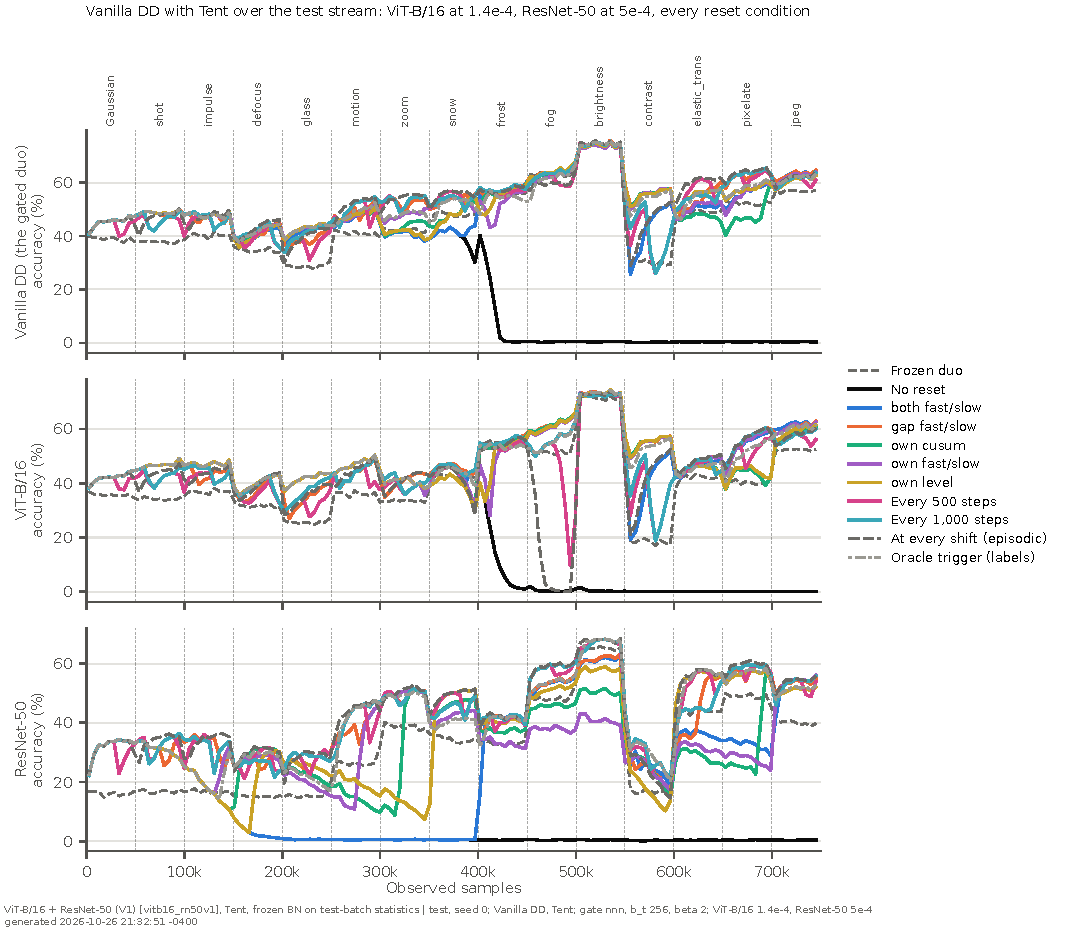
\includegraphics[width=\linewidth]{figures/reset_live/overlay_test_seed0.pdf}
  \caption{Test stream, seed 0: Vanilla DD (top), the \vit{} and the \rn{} (below) under every condition, accuracy over windows of 5,120 images; the dashed grey line is the frozen duo / member, dashed lines the references (episodic, oracle). Without a reset (black) both members die (accuracy below 5\% for four windows of 5,120 images): the \rn{} from 158,720 images, the \vit{} from 430,080. \rl{both\_fast\_vs\_slow} (blue) leaves the \rn{} at 0\% until about 400k.}
  \label{fig:overlay-test}
\end{figure}

\begin{figure}[t]
  \centering
  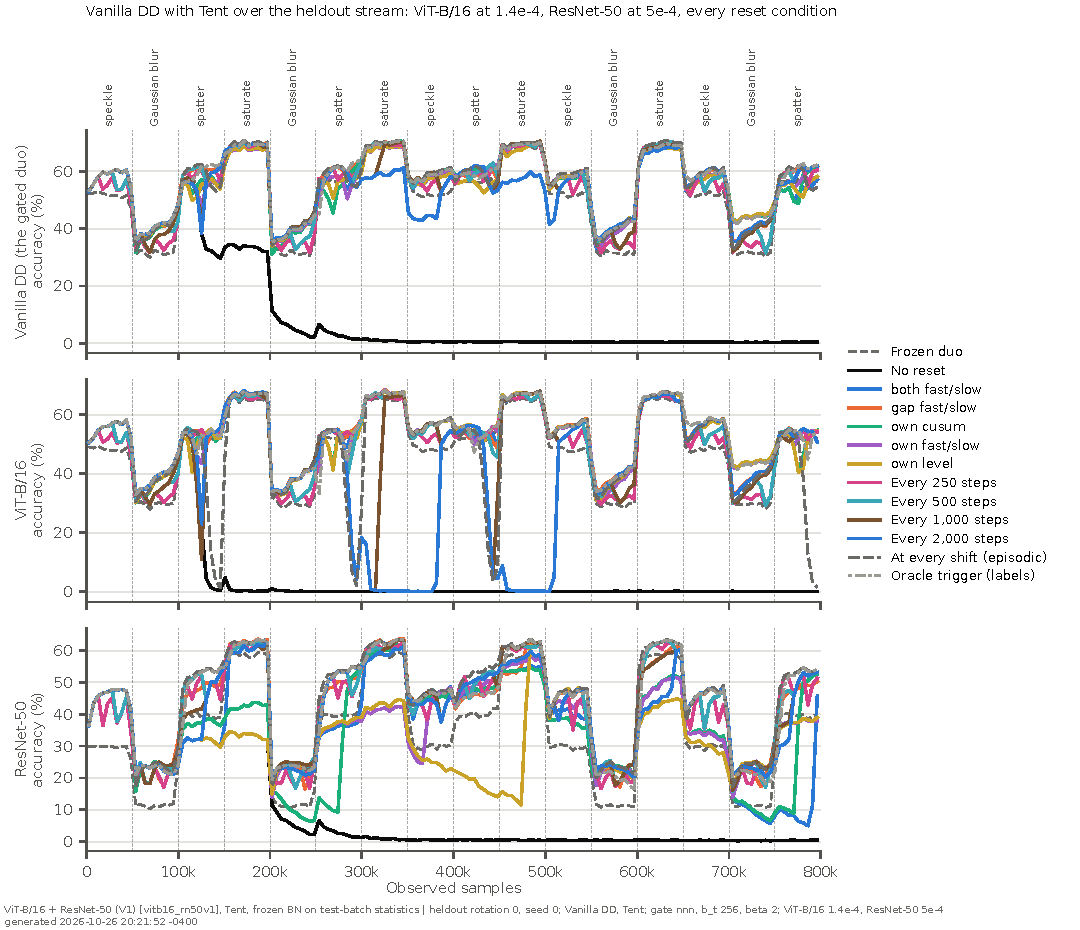
\includegraphics[width=\linewidth]{figures/reset_live/overlay_heldout_rot0.pdf}
  \caption{As Figure~\ref{fig:overlay-test} on the held-out stream (4 shifts $\times$ 4 rounds, rotation 0).}
  \label{fig:overlay-held}
\end{figure}

\begin{itemize}
  \item \textbf{The best rule is \rl{gap\_fast\_vs\_slow}} (56.5 held-out, 53.8 test). It beats every fixed schedule on both streams and the episodic reset on test (53.3), is 0.4 below the oracle on held-out and 1.2 above it on test.
  \item \textbf{The offline ranking carries to test.} The live order of the five leaders on test (53.8, 52.4, 51.8, 51.8, 50.9) is their offline order of Table~\ref{tab:b1}: \rl{gap}, \rl{own\_fast}, \rl{own\_cusum}, \rl{own\_level}, \rl{both\_fast\_vs\_slow}. On held-out the five are within 1.1 points (55.4--56.5) and \rl{both\_fast\_vs\_slow} is second.
  \item \textbf{\rl{both\_fast\_vs\_slow} fails on test.} It leaves the \rn{} below 5\% for 32\% of the stream (seed 0; the blue line of Figure~\ref{fig:overlay-test}), which the screen had flagged (it missed the \rn{} on test). The other four rules keep both members above 5\% for essentially the whole stream (at most 1\% of windows dead).
  \item \textbf{Oracle and episodic are not ceilings.} The oracle scores 52.6 on test, below \rl{gap}, the episodic reset and the 1,000-step schedule. The episodic reset lets the \vit{} collapse inside a single shift (fog) and it stays dead until the next boundary (Figure~\ref{fig:overlay-test}, middle panel).
  \item \textbf{Rules protect the \vit{}, schedules protect the \rn{}} (Table~\ref{tab:livemem}). On test the \vit{} scores 48.8--50.0 under the rules and 49.2 under the oracle, but 44.5--47.3 under the schedules and the episodic reset; the \rn{} scores 42.6--43.8 under those and 26.5--40.9 under the rules.
  \item \textbf{How often you reset matters.} The fixed periods score 54.3, 55.4, 55.3 and 53.5 on held-out for 250, 500, 1000 and 2000 steps: too frequent costs adaptation, too rare lets the collapse through. The held-out pick, 500, does not carry to test (51.7, against 52.7 for 1000).
  \item \textbf{At matched reset frequency} \rl{gap\_fast\_vs\_slow} (2--3 resets per 1,000 batches per member) beats the 1,000-step schedule (3.8) by 1.2 points on held-out and 1.1 on test. The own rules reset about 3 to 13 times less often than that schedule and land within it: $+0.1$ to $+0.4$ on held-out, $-0.3$ to $-0.9$ on test; \rl{both\_fast\_vs\_slow} is $-1.8$ on test.
  \item \textbf{The audit does not predict harm.} 91\% of \rl{gap}'s test resets are false (66\% on held-out), against 5\% for \rl{own\_cusum}, 0\% for \rl{own\_level} and 29\% for \rl{own\_fast}, yet \rl{gap} wins. Its resets alternate (Figure~\ref{fig:gap}): in each test seed all 18 \vit{} resets follow a \rn{} reset 20--69k images earlier. A plausible reading, not checked here, is that a reset member's proxy dips and recovers, which moves its partner's gap, so the rule acts partly as an emergent schedule.
\end{itemize}

\begin{table}[t]
  \centering\footnotesize\setlength{\tabcolsep}{5pt}
  \caption{The members' own accuracy (\%) over the whole stream in the live runs of Table~\ref{tab:live}; Frozen = the same members without adaptation.}
  \label{tab:livemem}
  \begin{tabular}{@{}l rr rr@{}}
    \toprule
    & \multicolumn{2}{c}{held-out} & \multicolumn{2}{c}{test} \\
    \cmidrule(lr){2-3} \cmidrule(lr){4-5}
    condition & \vit{} & \rn{} & \vit{} & \rn{} \\
    \midrule
    Frozen & 48.8 & 34.9 & 40.4 & 31.7 \\
    \midrule
    No reset & 5.1 & 11.6 & 23.8 & 5.8 \\
    \midrule
    \rl{gap\_fast\_vs\_slow} & 53.5 & 43.5 & 50.0 & 40.9 \\
    \rl{own\_fast\_vs\_slow} & 53.3 & 36.2 & 49.8 & 33.2 \\
    \rl{own\_cusum} & 53.2 & 35.8 & 48.9 & 34.3 \\
    \rl{own\_level} & 53.2 & 33.9 & 48.8 & 35.0 \\
    \rl{both\_fast\_vs\_slow} & 53.5 & 38.5 & 49.1 & 26.5 \\
    \midrule
    Every 250 steps & 50.7 & 42.5 & -- & -- \\
    Every 500 steps & 51.5 & 43.9 & 44.8 & 42.6 \\
    Every 1,000 steps & 48.6 & 43.9 & 47.3 & 42.6 \\
    Every 2,000 steps & 39.5 & 42.0 & -- & -- \\
    \midrule
    Episodic (every shift) & 49.0 & 45.7 & 44.5 & 43.8 \\
    Oracle (labels) & 53.7 & 44.2 & 49.2 & 40.8 \\
    \bottomrule
  \end{tabular}
\end{table}

\begin{figure}[t]
  \centering
  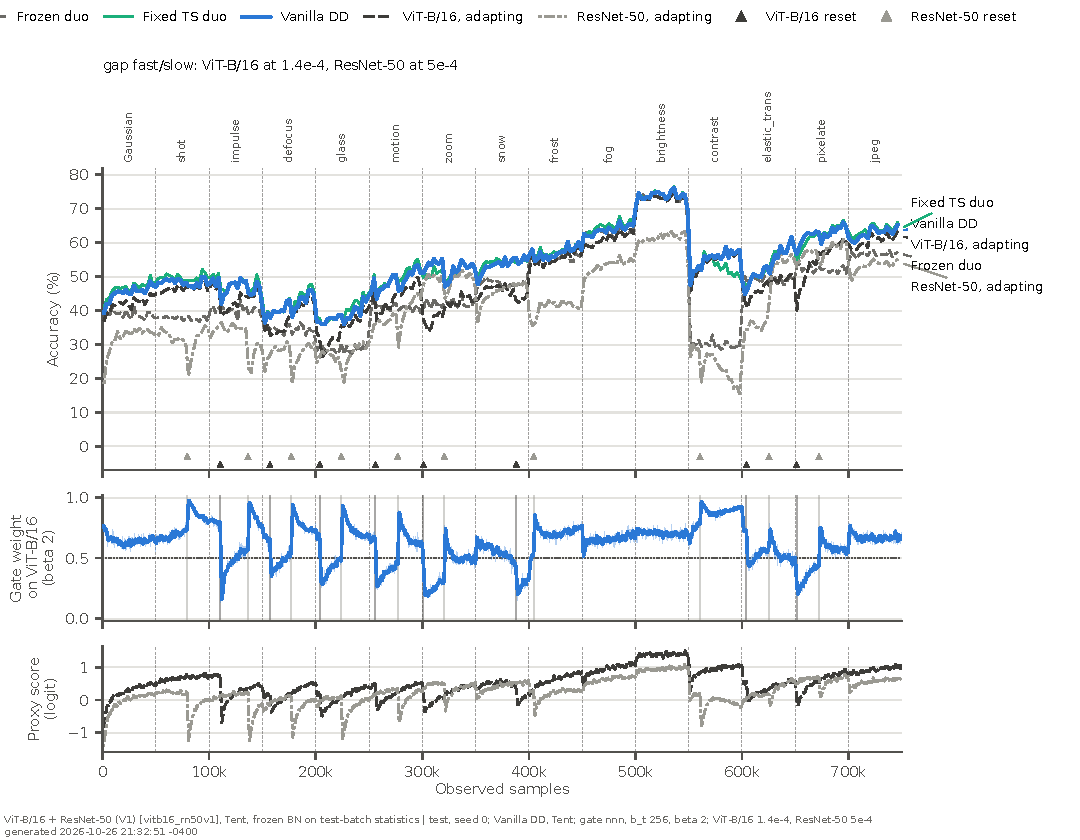
\includegraphics[width=0.92\linewidth]{figures/reset_live/gap_fast_vs_slow_test_seed0.pdf}
  \caption{\rl{gap\_fast\_vs\_slow}, test stream, seed 0: accuracy of the frozen duo, the fixed-TS duo, Vanilla DD and both members; the gate's weight on the \vit{}; the proxy scores it reads. A triangle marks each reset (dark: \vit{}, light: \rn{}), a line the same reset in the weight panel. The \rn{} is reset first and the \vit{} 20--69k images later, six times in a row in the first 400k images.}
  \label{fig:gap}
\end{figure}

\begin{figure}[t]
  \centering
  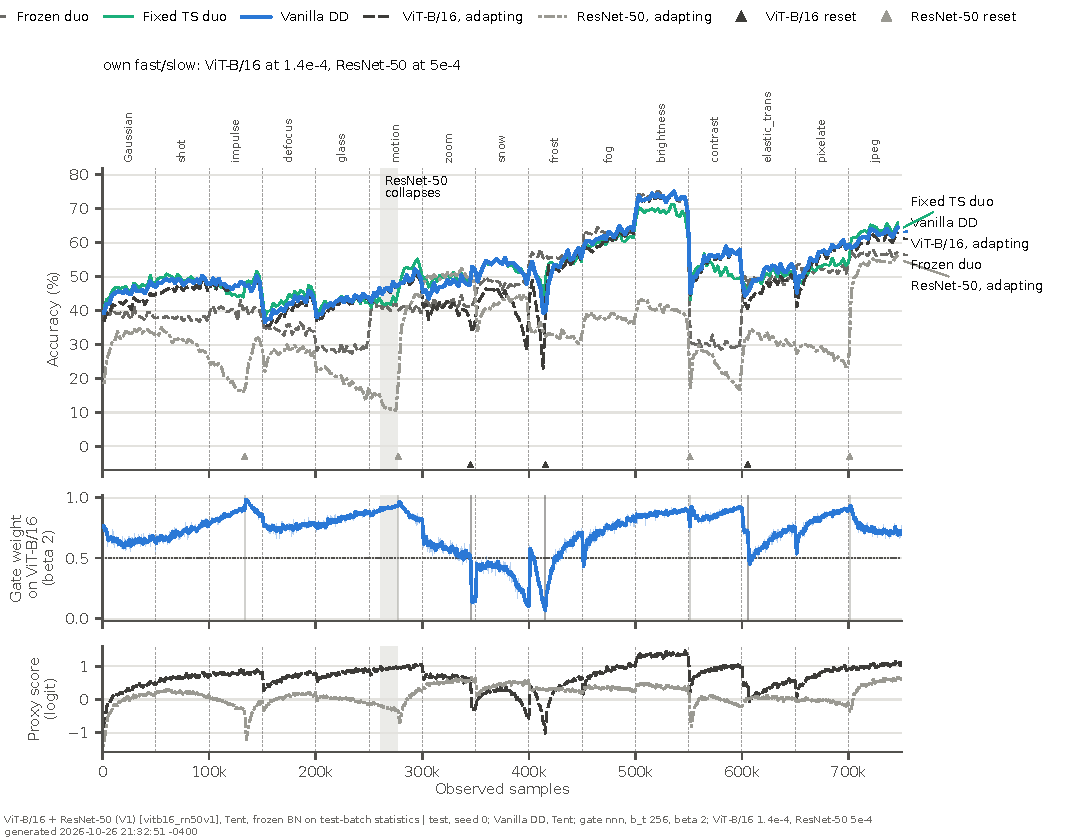
\includegraphics[width=0.92\linewidth]{figures/reset_live/own_fast_vs_slow_test_seed0.pdf}
  \caption{\rl{own\_fast\_vs\_slow}, test stream, seed 0, as Figure~\ref{fig:gap}. It resets far less often: seven resets in all, the \rn{} at 133k, 278k, 551k and 701k images and the \vit{} at 345k, 415k and 605k; the shaded band is the \rn{}'s collapse episode, reset at 278k. Between 278k and 551k the \rn{} is not reset.}
  \label{fig:own}
\end{figure}

\paragraph{What this does and does not show.} At fixed stress rates, whether a reset helps depends on how often it happens as much as on whether it follows a collapse, so the comparison mixes detection with reset frequency. What the runs support: the label-free rules rescue the duo from a collapse that costs 22 points against the frozen duo on test, match or beat the best blind schedule (the \rl{gap} rule by about 1 point, the own rules within 1 point with far fewer resets), and the offline screen predicted the live order on the test stream. They do not show that the rules detect collapses better than a schedule would at its own best rate.

\section{Limits and next steps}
\begin{itemize}
  \item \textbf{Little independent data.} The calibration pool has 4 independent rotations (the two seeds of a rotation are nearly identical) plus 2 healthy streams; T is 3 seeds of one stream. At budget 1 the pool allows about 32 false alarms in total, so differences of about 20\% in delay between rules are not meaningful. The live runs add 2 held-out rotations (the same images in another order) and 3 test seeds (the same corruptions shuffled differently, with deterministic models), so their small spreads reflect the data order only; differences below about 1 point are not meaningful.
  \item \textbf{Held-out is in-sample.} The rule settings (and the schedule period 500) were chosen on it; only the test stream is an honest comparison.
  \item \textbf{Fixed stress rates confound detection and reset frequency} (the main limit, see above). The next test is to tune each rule's rates with the rule running, on the held-out stream (a ladder of rates per rule), and to compare rules and schedules at matched reset counts. This is not run and needs a decision (roughly 30--40 GPU-hours).
  \item \textbf{The \rl{gap} mechanism} (a reset member's proxy dip moving its partner's gap) is a reading of the figures, not a measurement.
  \item \textbf{Grid edges.} The selected own and gap \rl{fast\_vs\_slow} settings sit on the lowest threshold of the grid ($\delta = 1$, at 0.69 and 0.91 false alarms, below the budget), and \rl{own\_cusum} on the lowest $\nu$ and $h$. The best setting may lie beyond the grid; the gap and both versions of cusum need a higher threshold range.
  \item \textbf{Short dips.} They account for most misses of the screen. Treating self-recovering dips under $\approx 32$ batches as non-events lowers every miss rate (for the leaders, from about $0.3$ to $0.2$) and could change the offline ranking.
  \item \textbf{Not yet run.} Joint DD with the best rule; the live rules at rates tuned for resetting; the oracle with other definitions.
\end{itemize}

\paragraph{Reproduce.}
\begin{itemize}
  \item \path{scripts/04c_gate_stress.py} writes the S, H and T runs (one call each, with \verb|--extra S:1.4e-4:5e-4|, \verb|--extra H:1.26e-5:2.2e-5|, \verb|--extra T:1.4e-4:5e-4 --stream test|).
  \item \path{scripts/37b_screen_resets_stress.py} (\verb|--duo vitb16_rn50v1 --bn|) runs the screen (CPU, about one minute) and writes \path{out/results/screen_resets_stress/}.
  \item \path{scripts/38_run_reset_live.py} runs the live conditions (GPU, about 70 minutes per run; \verb|--conditions|, \verb|--stream heldout|/\verb|test|), \path{scripts/39_tab_reset.py} writes the tables and figures of Section~\ref{sec:live}.
  \item Code: \path{src/reset/screening.py}, \path{detectors.py}, \path{controller.py}.
\end{itemize}

\end{document}
